%%%%%%%%%%%%%%%%%%%%%%%%%%%%%%%%%%%%%%%%%
% Jacobs Landscape Poster
% LaTeX Template
% Version 1.1 (14/06/14)
%
% Created by:
% Computational Physics and Biophysics Group, Jacobs University
% https://teamwork.jacobs-university.de:8443/confluence/display/CoPandBiG/LaTeX+Poster
% 
% Further modified by:
% Nathaniel Johnston (nathaniel@njohnston.ca)
%
% This template has been downloaded from:
% http://www.LaTeXTemplates.com
%
% License:
% CC BY-NC-SA 3.0 (http://creativecommons.org/licenses/by-nc-sa/3.0/)
%
%%%%%%%%%%%%%%%%%%%%%%%%%%%%%%%%%%%%%%%%%

%----------------------------------------------------------------------------------------
%	PACKAGES AND OTHER DOCUMENT CONFIGURATIONS
%----------------------------------------------------------------------------------------

\documentclass[final]{beamer}

\usepackage[scale=0.95]{beamerposter} % Use the beamerposter package for laying out the poster

\usetheme{confposter} % Use the confposter theme supplied with this template

\setbeamercolor{block title}{fg=ngreen,bg=white} % Colors of the block titles
\setbeamercolor{block body}{fg=black,bg=white} % Colors of the body of blocks
\setbeamercolor{block alerted title}{fg=white,bg=dblue!70} % Colors of the highlighted block titles
\setbeamercolor{block alerted body}{fg=black,bg=dblue!10} % Colors of the body of highlighted blocks
% Many more colors are available for use in beamerthemeconfposter.sty

%-----------------------------------------------------------
% Define the column widths and overall poster size
% To set effective sepwid, onecolwid and twocolwid values, first choose how many columns you want and how much separation you want between columns
% In this template, the separation width chosen is 0.024 of the paper width and a 4-column layout
% onecolwid should therefore be (1-(# of columns+1)*sepwid)/# of columns e.g. (1-(4+1)*0.024)/4 = 0.22
% Set twocolwid to be (2*onecolwid)+sepwid = 0.464
% Set threecolwid to be (3*onecolwid)+2*sepwid = 0.708

\newlength{\sepwid}
\newlength{\onecolwid}
\newlength{\twocolwid}
\newlength{\threecolwid}
\setlength{\paperwidth}{48in} % A0 width: 46.8in
\setlength{\paperheight}{36in} % A0 height: 33.1in
\setlength{\sepwid}{0.024\paperwidth} % Separation width (white space) between columns
\setlength{\onecolwid}{0.22\paperwidth} % Width of one column
\setlength{\twocolwid}{0.464\paperwidth} % Width of two columns
\setlength{\threecolwid}{0.708\paperwidth} % Width of three columns
\setlength{\topmargin}{-0.5in} % Reduce the top margin size
%-----------------------------------------------------------

\usepackage{graphicx}  % Required for including images

\usepackage{booktabs} % Top and bottom rules for tables


\title{Integer-Linear-Program based Inference \\
	for Elementary School Science Example Question Answering
	} % Poster title

%	\begin{center}
%		\begin{tabular}{ccc}
%			
\includegraphics[width=0.4\linewidth]{logo.png} & \hfill & 
\includegraphics[width=0.4\linewidth]{logo.png}
%		\end{tabular}
%	\end{center}

\author{Daniel Khashabi$^*$, Ashish Shabrawal$^a$, Tushar Khot$^a$, 
	Peter Clark$^a$, Peter Turney$^a$, Oren Etzioni$^a$, Dan Roth$^*$} 

\institute{Cogntive Computation Group, UIUC$^*$ \quad \quad Allen Institute for Artificial Intelligence$^a$ 
	 } 

%\begin{figure}
%	
\includegraphics[scale=0.4]{logo.png}
%\end{figure}

\begin{document}

\addtobeamertemplate{headline}{} 
{
	\begin{tikzpicture}[remember picture,overlay] 
	\node [shift={(-11.5 cm,-6.0cm)}] at (current page.north east) {
\includegraphics[scale=0.9]{ai2.png}}; 
	\node [shift={(11 cm,-7cm)}] at (current page.north west) {
\includegraphics[scale=2.7]{ccg.png}}; 
	\end{tikzpicture} 
}

\addtobeamertemplate{block end}{}{\vspace*{2ex}} % White space under blocks
\addtobeamertemplate{block alerted end}{}{\vspace*{2ex}} % White space under highlighted (alert) blocks

\setlength{\belowcaptionskip}{2ex} % White space under figures
\setlength\belowdisplayshortskip{2ex} % White space under equations

\begin{frame}[t] % The whole poster is enclosed in one beamer frame

\begin{columns}[t] % The whole poster consists of three major columns, the second of which is split into two columns twice - the [t] option aligns each column's content to the top

\begin{column}{\sepwid}\end{column} % Empty spacer column

\begin{column}{\onecolwid} % The first column

\begin{block}{Introduction}

	\setbeamercolor{block alerted title}{fg=white, bg=white} % Colors of the highlighted block titles
	\setbeamercolor{block alerted body}{fg=black,bg=dblue!10} % Colors of the body of 

\begin{itemize}
	\item Elementary Science tests, a grand challenge for AI because of the wide variety	of knowledge and reasoning skills required. 
	\item Fourth Grade test-taking requires question answering (QA) that goes significantly beyond retrieval techniques, yet is simple enough to be accessible.
	\item In a sense, it is a simple embodiment of an AI challenge
	requiring both language and reasoning, suitable as part
	of a broader Turing Test
	\vspace{-0.5cm}
	\begin{alertblock}{}
		\footnotesize
		Fourth graders are planning a roller-skate race. Which
		surface would be the best for this race? (A) gravel (B) sand (C) blacktop (D) grass
	\end{alertblock} 
	\vspace{-1cm}
	Multiple ways to answer this question: 
	\begin{enumerate}
		\item There may be a sentence on the Web that happens to state the answer
		explicitly (e.g., ``Blacktop is a good surface for a rollerskating
		race''), and could be reliably retrieved to support the
		correct answer (``blacktop''). 
		\item Corpus statistics may reveal that ``blacktop'' is strongly associated with ``roller skating'' and ``race'', indicating that blacktop is the right answer.
		\item We might infer the answer from more general knowledge, e.g., roller-skating requires a smooth surface, and blacktop has a smooth surface, therefore blacktop is good for roller-skating. { \color{blue}$\Rightarrow $ OUR FOCUS HERE! }
	\end{enumerate}
	\end{itemize}
\end{block}

	\begin{block}{Classes of Questions}
		Five classes of question that are hard for all of its constituent solvers to answer
		reliably, in the absence of a corpus sentence containing the answer explicitly:
		\begin{enumerate}
			\item Complex inference \\
			\textit{A white rabbit is best protected in (A) a snowy field..}
			\item Structured questions \\ 
			\textit{Which structure is correctly paired with its function? }
			\item Comparison questions \\
			\textit{ ...moves faster or slower than ...?}
			\item Simple arithmetic reasoning \\ 
			\textit{7 rotations of Earth equals (A) 1 week (B) 2 weeks}
			\item Story Questions \\ 
			\textit{A puddle formed. Then the sun came out ...}
		\end{enumerate}
		We hope to solve the first two classes here. 
	\end{block}
	
	\begin{block}{Knowledge Representation}
		\begin{itemize}
			\item The ILPsolver uses knowledge represented as a set of tables
			\item Each knowledge table $T$ consists of a head-body pair $(H_T ,B_T )$ and captures a relation or predicate $R_T(x_1, \hdots, x_n )$ defined over entities.
			\item Columns of $T$ represent attributes of $R_T$ with attribute names in the header row $H_T$ , rows of $T$ represent $n$-tuples or instances
			of $R_T$ , and cells of $T$ represent entities as natural language
			phrases.
			\item Tables were built using an interactive table-building tool
			applied to science texts. The tool performs bootstrapped relation extraction over a corpus, with a user in the loop to
			suggest syntactic patterns and accept/reject matches, allowing tables to be built quickly.
		\end{itemize}	
	\end{block}

\end{column} % End of the first column

\begin{column}{\sepwid}\end{column} % Empty spacer column

\begin{column}{\twocolwid} % Begin a column which is two columns wide (column 2)

\begin{columns}[t,totalwidth=\twocolwid] % Split up the two columns wide column

\begin{column}{\onecolwid}\vspace{-.6in} % The first column within column 2 (column 2.1)

\begin{block}{Proof Structure}
\begin{itemize}
	\item Informally, question-answering involves matching lexical
	chunks in the question $q$ and answer option $a_i$ against one or
	more table rows, or a chain of joined rows, and returning the
	strength of that match as the confidence in $a_i$. 
	\item For example, a path through multiple joined rows is shown in {\color{blue} the blue box}. 
	\item We call such connections, which in general form
	a connected \textit{graph structure}, a proof graph, and question-answering involves selecting the answer option with the best
	scoring proof graph. 
	\item Matching is not just string equality, as there may be lexical variation among question	chunks and table cells (e.g., ``fall'' vs. ``autumn'').
\end{itemize}
\end{block}

\begin{block}{ILPsolver: Preliminaries}	
\begin{itemize}
	\item Formally, we treat this task as a discrete global optimization problem over tables. 
	\item Let $T$ be a set of knowledge tables and $g(t,h)$ be a (possibly directional) similarity measure in $[0,1]$ between short natural
	language phrases $t$ and $h$. 
	\item  Let $q$ denote a multiple choice	question with answer options $A = \{a_i \}_i$ and correct answer $a^* \in A$. 
	\item We build an ILP model $M = M(q,A,T)$ over a set $V$ of integer-valued variables, a set $C$ of linear constraints over $V$ and a linear maximization objective function $f = f(q,A,T )$ whose maximizer can be easily mapped to a candidate answer, ideally $a^*$. 
	\item At a high level, $M$ defines the space of possible proof graphs or reasoning patterns that ``connect'' lexical chunks of $q$ with some answer option a $i \in A$ through cells in one or more tables in $T$.
\end{itemize}

\end{block}

%----------------------------------------------------------------------------------------

\end{column} % End of column 2.1

\begin{column}{\onecolwid}\vspace{-.6in} % The second column within column 2 (column 2.2)

\begin{block}{ILPsolver: Model}
	\textbf{Variables:} $V$ define possible connections or edges between
	lexical chunks in $q$, answer options $A$, and cells of tables $T$. To improve scalability and reduce noise, we use the top few (typically 4-6) tables matching $q$ as ranked by a  simple TF-IDF scoring mechanism. \\
	\textbf{Constraints:} 
	Constraints $C$ reduce the exponentially large search space
	to proof graphs to what a human might consider as meaningful and appropriate for elementary science reasoning.
	The constraints are designed from manual
	inspection of desirable proof graphs. Although manually
	built, they are not specific to 4th Grade Science so are a
	one-time cost. Here are a few important constraints: 
\begin{itemize}
	\small 
	\item At most $1$ active rows  from each table. 
	\item At least $2$ constituents of the question must be active! 
\end{itemize}
	\textbf{Objective:} The objective function $f$ associates with every feasible
	proof graph $P$ a score $f_P$ designed to balance rewards (such as for including many links with high similarity	measure $g$ or linking with more columns of a table) with penalties (such as for using too many tables or low similarity links).

	%\begin{block}{Result and Analysis}
	\begin{table}
		{ \small
		\begin{tabular}{|c|c|c|c|}
			\hline 
			Solver & Train   & Test & Run time (on Train) \\ 
			\hline 
			\hline 
			\shortstack{ILPsolver \\ (with Lucene fallback)}  &  80.60\% & -- & \shortstack{ 2 minutes\\ 36 seconds} \\ 
			\hline 
			ILPsolver  &  72\% & 43.8\% & -- \\ 
			\hline 
		\end{tabular}
		}
	\end{table}
		
		\begin{itemize}
			\item Relative strength is for questions where multiple pieces of information need to be combined together. 
			\item Successfully answers the following by joining two rows of two different tables together: \\
			{\tt 
				table13:has-part(``plant'', ``stomata'').
				tablez3:part-output(``stomata'', ``oxygen'').
			} 
			\\
			{\small  \textit{ Which gas is given off by plants? (A) Hydrogen (B) Nitrogen (C) Oxygen (D) Helium} }
			\item In contrast, the PMI solver and the RULE solver both answer
			this question incorrectly: plants and nitrogen have high
			co-occurrence, and the RULE solver does not have an appropriate
			rule.
		\end{itemize}		
	%\end{block}
\end{block}

\end{column} % End of column 2.1

\end{columns} % End of the split of column 2 - any content after this will now take up 2 columns width

\begin{alertblock}{An example proof graph}
\begin{figure}
	\centering
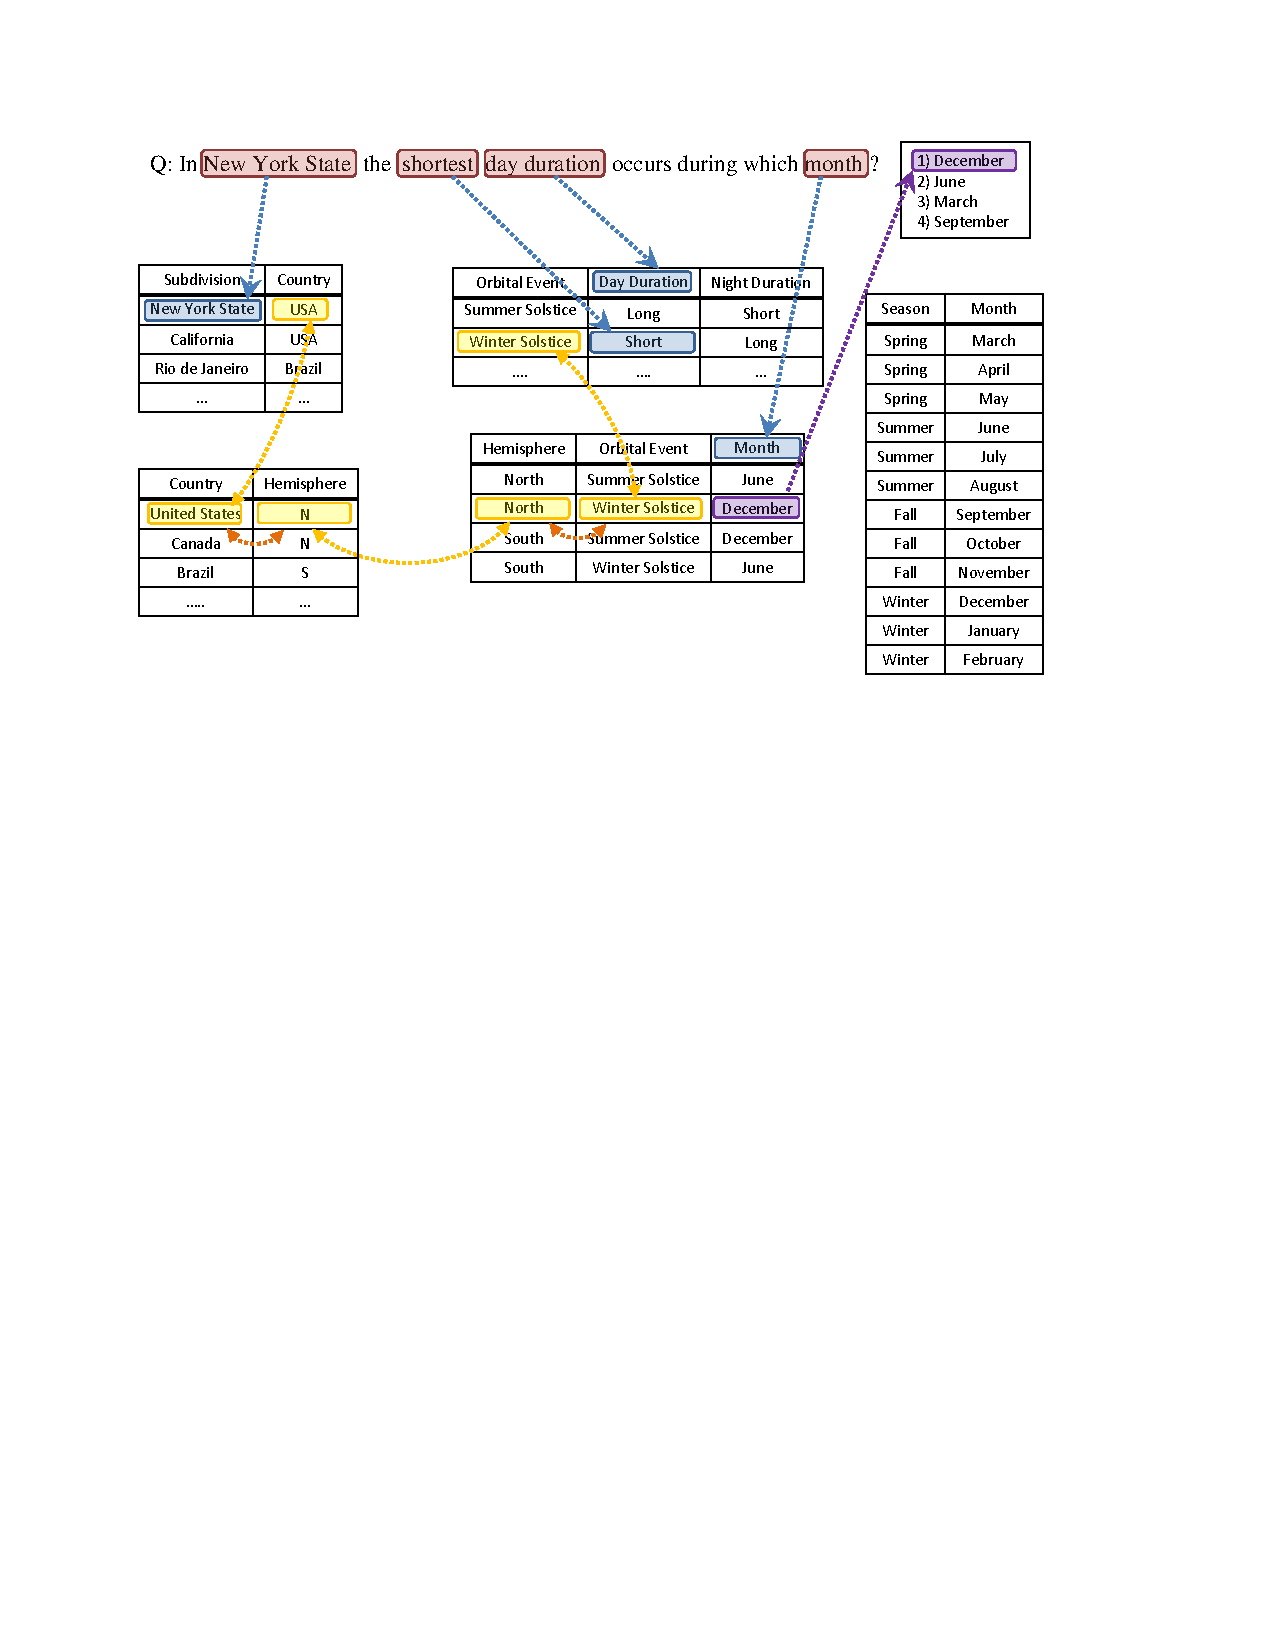
\includegraphics[trim=0.0cm 16.2cm 1cm 2.3cm,clip=true, scale=2.4]{newyorkQ.pdf}	
\end{figure}

\end{alertblock} 


\begin{columns}[t,totalwidth=\twocolwid] % Split up the two columns wide column again

\begin{column}{\onecolwid} % The first column within column 2 (column 2.1)


\end{column} % End of column 2.2

\end{columns} % End of the split of column 2

\end{column} % End of the second column

\begin{column}{\sepwid}\end{column} % Empty spacer column

\begin{column}{\onecolwid} % The third column

\begin{block}{}
		Two main failure modes:
		\begin{enumerate}
			\item Missing knowledge: The curated tables do not cover the
			information required.
			\item Control: While the table solver uses global constraints to
			constrain the paths explored, it may still find nonsensical
			paths (joins) through the tables during inference.
		\end{enumerate}
\end{block}

\begin{block}{Combination Solver}
Five solvers, each using different types of knowledge, to answer multiple choice questions.
\begin{figure}
	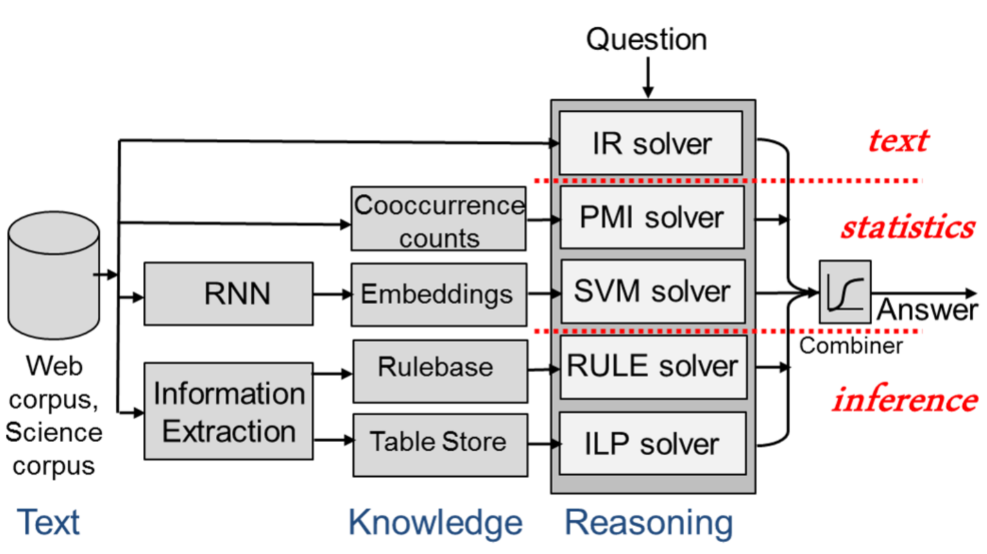
\includegraphics[scale=0.8]{combination.png}
\end{figure}
\begin{itemize}
	\item The IR solver operates directly on the text. The
	PMI solver and the SVM solver use statistical data derived
	from text.
	\item  The RULE solver and the ILP solver reason with
	knowledge extracted from text. 
	\item Each solver assigns confidences to each of the answer options, and a combiner module combines the results together using logistic regression
	trained on a set of training examples.
\end{itemize}

\begin{figure}
	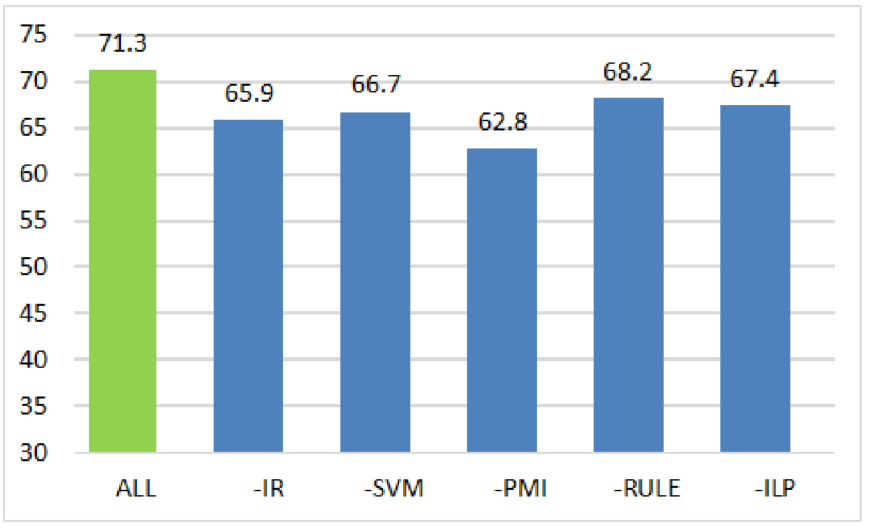
\includegraphics[scale=0.9]{ablation.png}
	\hspace{0.5cm}
	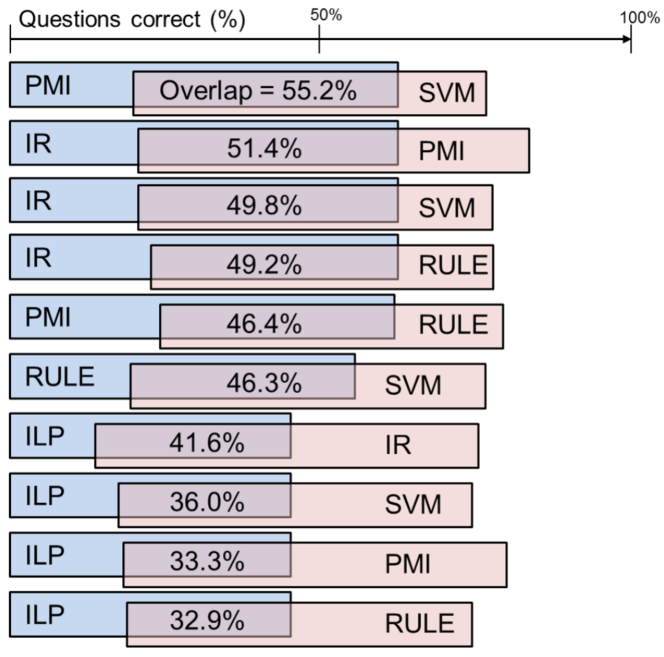
\includegraphics[scale=0.9]{solverPairs.png}
\end{figure}

\begin{itemize}
	\item Figure left: Effect of removing an individual solver from the ensemble. The results suggest each solver contributes to the overall score 
	\item Figure right: Different pairs of solvers answer substantially different question sets correctly (i.e., solvers are not redundant with each other).
\end{itemize}

\end{block}


\begin{block}{Selected References}

\nocite{*} 
\small{\bibliographystyle{unsrt}
\bibliography{sample}\vspace{0.75in}}

\end{block}

\setbeamercolor{block title}{fg=red,bg=white} % Change the block title color

\vspace{-2	cm}

\begin{block}{Acknowledgements}
	\footnotesize{
	DK is supported partly by Google and Allen Institute for Artificial Intelligence.  
	We are also grateful to Christos Christodoulopoulos, Sujay Jauhar, Niranjan Balasubramanian, Sumithra Bhakthavatsalam, Isaac Cowhey, Dirk
	Groeneveld, Kevin Humphreys, Jesse Kinkead, Roie Levin,
	Carissa Schoenick and Sam Skjonsberg for their contributions to this work. 
	}
\end{block}

\end{column} % End of the third column

\end{columns} % End of all the columns in the poster

\end{frame} % End of the enclosing frame

\end{document}
